\documentclass[11pt,a4paper]{article}
\usepackage[margin=25mm]{geometry}
\usepackage{graphicx}
\usepackage{amsmath}
\usepackage{booktabs}
\usepackage{array}
\usepackage{float}
\usepackage{tabularx}
\usepackage{enumitem}
\setlist{itemsep=2pt,topsep=3pt,parsep=0pt}
\setlength{\emergencystretch}{1em}
\graphicspath{{figures/}}
\newcolumntype{Y}{>{\raggedright\arraybackslash}X}

\title{High-Temperature Heat Pump Cycle Comparison:\\Baseline (S0) vs.\ Internal Heat Exchanger Cycle (S4)}
\author{Project Report}
\date{}

\begin{document}
\maketitle

\noindent\textbf{Scope of this draft.} This document explains the systems and assumptions that we propose to implement. It sets out the physical model and the planned analysis; it does not present completed simulations or performance results. The final report, including results, will remain within 10 pages.

\section{What we propose to study}

\subsection{The purpose of the heat pump}
Our system will recover heat from an industrial waste-water stream and use it to heat a second water stream to $130\,^\circ\mathrm{C}$. The source water is only at $35\,^\circ\mathrm{C}$, so it cannot heat the sink water directly. A heat pump makes this transfer possible by circulating a refrigerant and supplying mechanical work to a compressor.

We will compare two arrangements from the project specification~\cite{assignment}. The first, \textbf{S0}, is a standard cycle with a compressor, condenser, expansion valve and evaporator. The second, \textbf{S4}, adds an \textbf{internal heat exchanger (IHX)} between two parts of the same refrigerant circuit. We want to understand how this addition changes the heat exchanged inside the cycle, the required exchanger areas, the heating efficiency and the compressor discharge temperature.

\subsection{Three separate fluid circuits}
There will be three circuits. The fluids exchange heat through exchanger walls; they do not mix.
\begin{itemize}
    \item \textbf{Source-water circuit:} waste-heat water enters the evaporator at $35\,^\circ\mathrm{C}$ and leaves at $30\,^\circ\mathrm{C}$. Its temperature falls because it gives heat to the refrigerant.
    \item \textbf{Refrigerant circuit:} R1233zd(E) circulates in a closed loop. It absorbs heat at low pressure, is compressed, releases heat at high pressure, and is expanded back to low pressure.
    \item \textbf{Sink-water circuit:} pressurized water enters the condenser at $120\,^\circ\mathrm{C}$ and leaves at $130\,^\circ\mathrm{C}$. This heating is the useful output of the system.
\end{itemize}
The words \emph{source} and \emph{sink} describe where heat comes from and where it is delivered. Although called the source, the waste-water stream is colder than the sink-water stream. The evaporator and condenser are named for what happens to the \emph{refrigerant}, not to the water.

\begin{figure}[H]
    \centering
    \begin{minipage}[t]{0.48\textwidth}
        \centering
        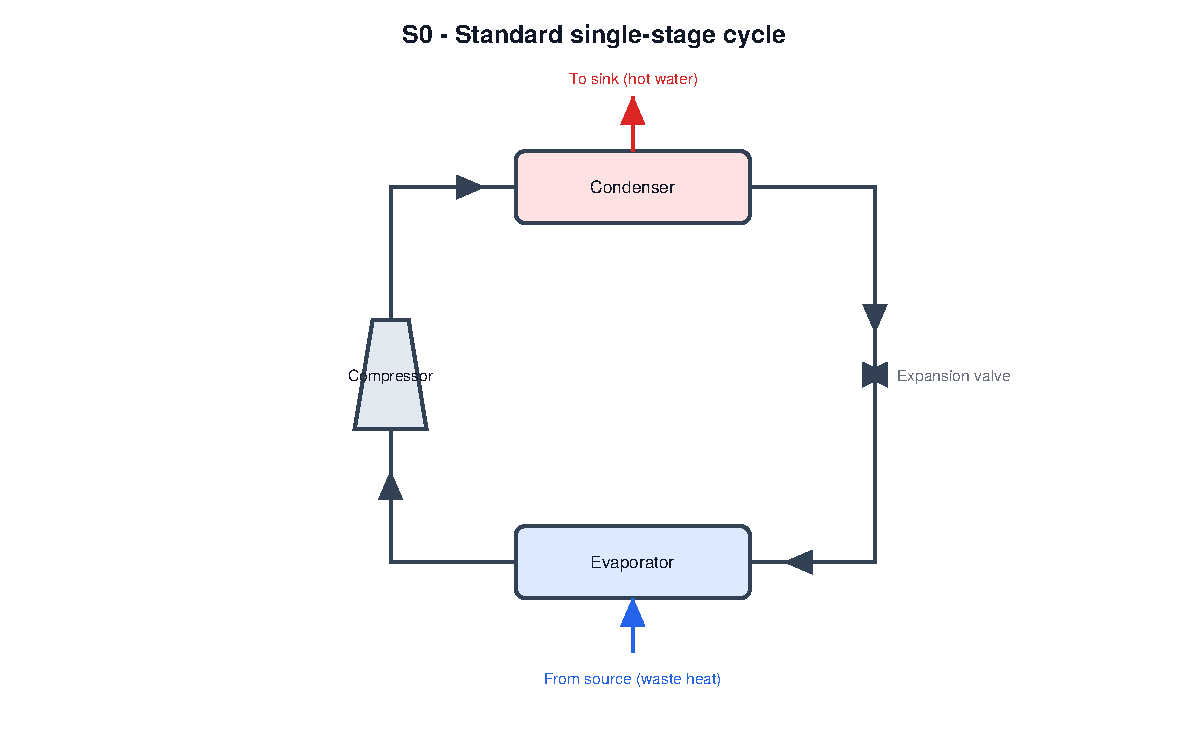
\includegraphics[width=\textwidth]{hp_s0.pdf}
        \caption{S0: standard single-stage cycle.}
        \label{fig:s0}
    \end{minipage}\hfill
    \begin{minipage}[t]{0.48\textwidth}
        \centering
        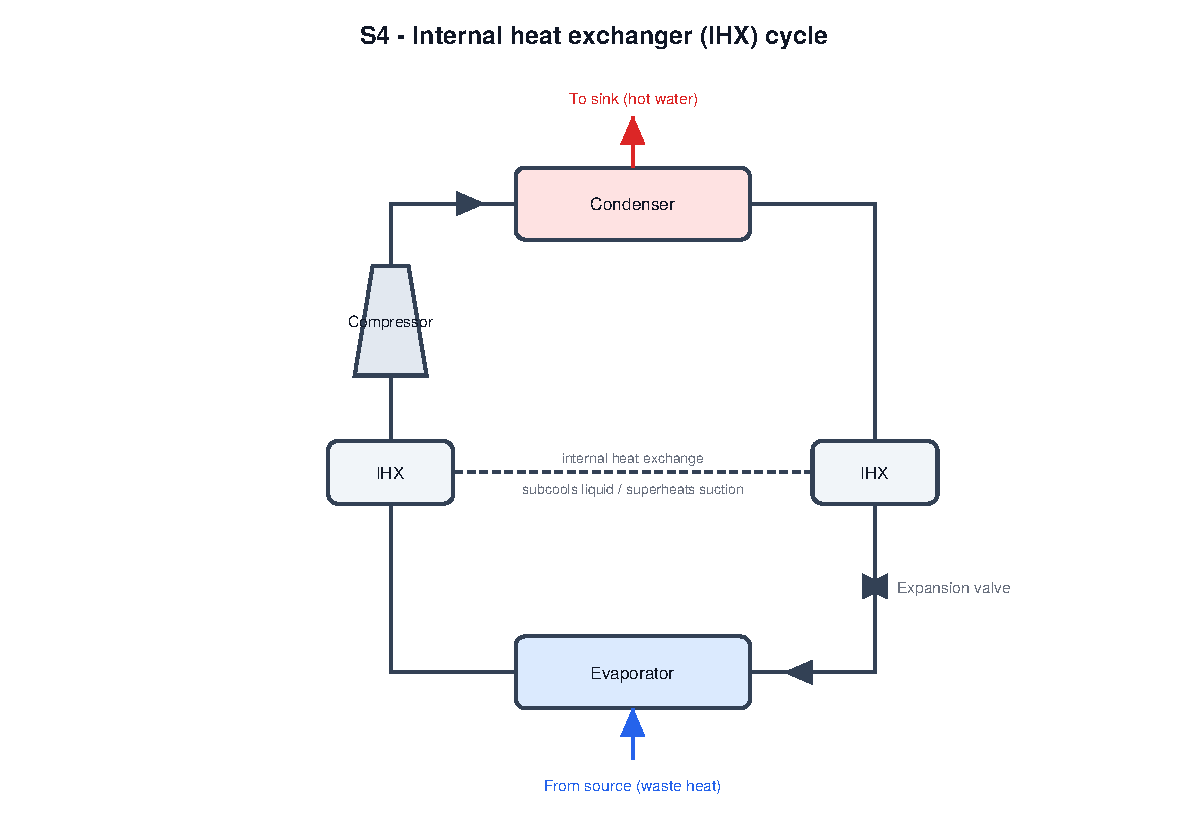
\includegraphics[width=\textwidth]{hp_s4.pdf}
        \caption{S4: cycle with internal heat exchange.}
        \label{fig:s4}
    \end{minipage}
\end{figure}

\section{Common operating conditions and assumptions}

\subsection{The conditions we will impose}
Both cycles will deliver the same useful heating power, $\dot Q_{\mathrm{cond}}=100\,\mathrm{kW}$, under the same water temperatures and pressures. This common basis is essential: a difference in performance should come from the cycle arrangement or its chosen parameters, rather than from a different heating task.

\begin{table}[H]
\centering
\caption{Prescribed nominal conditions, following the assignment.}
\label{tab:inputs}
\small
\begin{tabularx}{\textwidth}{@{}>{\raggedright\arraybackslash}p{4.7cm}>{\raggedright\arraybackslash}p{3.7cm}Y@{}}
\toprule
Quantity & Value & Meaning \\
\midrule
Refrigerant & R1233zd(E) & Same fluid in S0 and S4 \\
Condenser heating duty & $100\,\mathrm{kW}$ & Useful heat delivered to sink water \\
Sink water & $120\to130\,^\circ\mathrm{C}$; $10\,\mathrm{bar}$ & Liquid water heated in condenser \\
Source water & $35\to30\,^\circ\mathrm{C}$; $3\,\mathrm{bar}$ & Liquid water cooled in evaporator \\
Saturation-temperature approach & $5\,\mathrm{K}$ & Sets the nominal pressure levels \\
Compressor isentropic efficiency & $0.70$ & Same in both cycles \\
Condenser outlet subcooling & $5\,\mathrm{K}$ & Applies before the IHX in S4 \\
S0 evaporator outlet superheat & $5\,\mathrm{K}$ & Sets S0 compressor inlet state \\
S4 evaporator outlet quality & $x_{\mathrm{evap}}=0.90$ & Nominal vapour mass fraction \\
S4 compressor inlet superheat & $\Delta T_{\mathrm{suc}}=5\,\mathrm{K}$ & Measured after the IHX \\
Film coefficients, each side & $3000\,\mathrm{W/(m^2 K)}$ & Water and refrigerant; all exchangers \\
Cold-side to hot-side area ratio & $1:1$ & Equal surface areas on both sides \\
\bottomrule
\end{tabularx}
\end{table}

\subsection{How the pressure levels will be chosen}
The assignment fixes the refrigerant saturation temperatures using the water outlet temperatures and a $5\,\mathrm{K}$ approach:
\begin{align}
T_{\mathrm{cond}} &= 130\,^\circ\mathrm{C}+5\,\mathrm{K}=135\,^\circ\mathrm{C},\\
T_{\mathrm{evap}} &= 30\,^\circ\mathrm{C}-5\,\mathrm{K}=25\,^\circ\mathrm{C}.
\end{align}
CoolProp will give the corresponding saturation pressures for R1233zd(E): approximately $20.99\,\mathrm{bar}$ and $1.30\,\mathrm{bar}$, respectively. These are the high and low pressures of the refrigerant circuit. The water pressures of 10 and 3 bar belong to separate circuits and do not set the refrigerant pressures.

The stated $5\,\mathrm{K}$ rule is a convention for selecting the saturation levels. Actual refrigerant inlet and outlet temperatures also depend on superheat and subcooling. We will therefore check the exchanger terminal temperature differences separately; the single-zone approximation will not resolve the minimum temperature difference everywhere inside each exchanger.

\subsection{What superheat, subcooling and quality mean}
At a given pressure, the saturation temperature is the temperature at which a pure fluid can change between liquid and vapour. \textbf{Superheat} means that vapour is warmer than this saturation temperature. \textbf{Subcooling} means that liquid is colder than it.

For S0, the prescribed values give a compressor inlet temperature of $25+5=30\,^\circ\mathrm{C}$ and a condenser liquid outlet temperature of $135-5=130\,^\circ\mathrm{C}$. In S4, the condenser still delivers liquid at $130\,^\circ\mathrm{C}$, but the IHX cools it further before the expansion valve.

\textbf{Vapour quality}, $x$, is the fraction of the refrigerant mass that is vapour in a liquid--vapour mixture. Thus $x_{\mathrm{evap}}=0.90$ means 90\% vapour and 10\% liquid by mass, not by volume. At the low pressure, this mixture is at $25\,^\circ\mathrm{C}$. In S4 it will enter the IHX, where the remaining liquid must evaporate before the refrigerant becomes superheated vapour suitable for compression.

\subsection{Simplifications and their consequences}
We will use the following assumptions consistently for both cycles:
\begin{enumerate}
    \item \textbf{Steady state.} Temperatures, pressures and mass flows will be constant in time. We will study operating points, without simulating start-up, control behaviour or thermal storage.
    \item \textbf{Design sizing.} Heating duty and operating conditions will be prescribed, and the model will calculate the necessary mass flows and exchanger areas. This is not a prediction of how one fixed installed exchanger performs under changing loads.
    \item \textbf{No heat loss to the surroundings.} The compressor and external pipework will be adiabatic. Heat will pass only between the intended exchanger streams. The IHX will transfer heat internally, without adding energy from outside the heat pump.
    \item \textbf{No pressure losses in exchangers or pipes.} The refrigerant will have one high-pressure level and one low-pressure level. The compressor raises pressure and the valve lowers it. This simplifies the comparison but omits a possible penalty of adding a real IHX.
    \item \textbf{Single-zone counter-flow exchangers.} We will use the supplied \texttt{SizingHX} component for the condenser, evaporator and IHX, as required. The assignment describes this as a constant-$c_p$, single-zone approximation, including across phase changes. In the library, heat duties use real-fluid enthalpy differences, while area sizing uses one log-mean temperature difference based on the stream endpoints. We will not resolve separate liquid, two-phase and vapour zones. Areas will therefore be approximate comparison measures.
    \item \textbf{Constant film coefficients and equal side areas.} Each film coefficient will remain $3000\,\mathrm{W/(m^2 K)}$, independent of phase or flow rate. Wall and fouling resistances will be neglected. This gives a consistent sizing basis, without attempting a detailed exchanger design.
    \item \textbf{Adiabatic compression with fixed efficiency.} A constant isentropic efficiency of 0.70 will relate the actual enthalpy rise to an ideal isentropic compression. Discharge temperature will be calculated, not imposed. Compressor maps, motor losses and operating limits will not be modelled unless introduced explicitly later.
    \item \textbf{Isenthalpic expansion.} The valve will lower pressure without shaft work or heat transfer, so its inlet and outlet specific enthalpies will be equal. Part of the liquid can evaporate during this pressure drop.
    \item \textbf{Other energy terms.} Changes in kinetic and potential energy will be neglected. Reported input power will be compressor shaft power; water-pump and other auxiliary consumption will not be included.
\end{enumerate}

\section{How each proposed cycle will work}

\subsection{S0: the baseline cycle}
The refrigerant will pass through four components in this order:
\begin{enumerate}
    \item \textbf{Compressor:} low-pressure superheated vapour enters at state 1. Mechanical work raises its pressure and enthalpy. High-pressure vapour leaves at state 2.
    \item \textbf{Condenser:} the refrigerant releases heat to the sink water, condenses and becomes subcooled liquid. It leaves at state 3, at $130\,^\circ\mathrm{C}$.
    \item \textbf{Expansion valve:} the liquid pressure falls to the evaporation pressure at constant enthalpy. A liquid--vapour mixture leaves at state 4.
    \item \textbf{Evaporator:} the mixture absorbs heat from the source water. The liquid evaporates and the vapour gains $5\,\mathrm{K}$ of superheat, returning to state 1.
\end{enumerate}

\begin{table}[H]
\centering
\caption{Proposed S0 state numbering. Specific enthalpy is denoted by $h$.}
\small
\begin{tabularx}{\textwidth}{@{}c>{\raggedright\arraybackslash}p{5cm}Y@{}}
\toprule
State & Location & How the state will be determined \\
\midrule
1 & Evaporator outlet / compressor inlet & $p_{\mathrm{evap}}$, $T_1=T_{\mathrm{evap}}+5\,\mathrm{K}$ \\
2 & Compressor outlet / condenser inlet & $p_{\mathrm{cond}}$ and compressor efficiency \\
3 & Condenser outlet / valve inlet & $p_{\mathrm{cond}}$, $T_3=T_{\mathrm{cond}}-5\,\mathrm{K}$ \\
4 & Valve outlet / evaporator inlet & $p_{\mathrm{evap}}$, $h_4=h_3$ \\
\bottomrule
\end{tabularx}
\end{table}

The same refrigerant mass flow will pass through every component. Once the states are known, the required heating duty will determine this flow. We will not choose an additional arbitrary refrigerant mass flow.

\subsection{S4: adding the internal heat exchanger}
S4 will retain the same compressor, condenser, valve and evaporator, and add a counter-flow IHX. Its hot side will carry the high-pressure liquid leaving the condenser. Its cold side will carry the low-pressure refrigerant leaving the evaporator. These two streams belong to the same closed loop but remain separated by a wall in the IHX.

The refrigerant path will be
\[
\text{compressor}\to\text{condenser}\to\text{IHX hot side}\to\text{valve}
\]
\[
\to\text{evaporator}\to\text{IHX cold side}\to\text{compressor}.
\]
The hot liquid will give up heat and become more subcooled. The cold mixture will receive this heat, finish evaporating, and then become superheated vapour. The IHX will therefore move part of the refrigerant heating from the external evaporator into an internal exchange process.

\begin{table}[H]
\centering
\caption{Proposed S4 state numbering, defined separately from S0.}
\small
\begin{tabularx}{\textwidth}{@{}c>{\raggedright\arraybackslash}p{5cm}Y@{}}
\toprule
State & Location & How the state will be determined \\
\midrule
1 & IHX cold outlet / compressor inlet & $p_{\mathrm{evap}}$, $T_1=T_{\mathrm{evap}}+\Delta T_{\mathrm{suc}}$ \\
2 & Compressor outlet / condenser inlet & $p_{\mathrm{cond}}$ and compressor efficiency \\
3 & Condenser outlet / IHX hot inlet & $p_{\mathrm{cond}}$, $T_3=T_{\mathrm{cond}}-5\,\mathrm{K}$ \\
4 & IHX hot outlet / valve inlet & $p_{\mathrm{cond}}$ and IHX energy balance \\
5 & Valve outlet / evaporator inlet & $p_{\mathrm{evap}}$, $h_5=h_4$ \\
6 & Evaporator outlet / IHX cold inlet & $p_{\mathrm{evap}}$, chosen quality $x_{\mathrm{evap}}$ \\
\bottomrule
\end{tabularx}
\end{table}

\subsection{What changes in the S4 specification}
For S0, the evaporator itself must supply the final $5\,\mathrm{K}$ of superheat. For S4, we will instead prescribe two quantities: the evaporator outlet quality $x_{\mathrm{evap}}$ and the compressor suction superheat $\Delta T_{\mathrm{suc}}$. These are the two parameters that we will vary later.

The nominal values will be $x_{\mathrm{evap}}=0.90$ and $\Delta T_{\mathrm{suc}}=5\,\mathrm{K}$. The IHX duty and its liquid outlet temperature will follow from these conditions and energy conservation. We will not independently prescribe an IHX effectiveness, area or additional liquid subcooling, because that would introduce extra conditions into this design-sizing problem.

\section{The balances we will implement}

\subsection{Compressor and refrigerant flow}
Specific enthalpy $h$ is the energy carried per unit mass of flowing fluid; multiplying an enthalpy difference by a mass flow gives a heat or power rate. We will use CoolProp to obtain enthalpy, entropy and temperature from each state.

For either cycle, state 1 will be the compressor inlet and state 2 its outlet. The ideal discharge enthalpy $h_{2s}$ will be evaluated at the high pressure and the inlet entropy $s_1$. The actual discharge enthalpy will satisfy
\begin{equation}
h_2=h_1+\frac{h_{2s}-h_1}{\eta_{\mathrm{is}}},
\qquad \eta_{\mathrm{is}}=0.70.
\end{equation}
A lower efficiency means a larger actual enthalpy rise for the same ideal compression. The discharge temperature will then follow from $(p_{\mathrm{cond}},h_2)$.

With state 3 at the condenser outlet in both cycles, the refrigerant flow will satisfy
\begin{equation}
\dot m_{\mathrm{ref}}=\frac{\dot Q_{\mathrm{cond}}}{h_2-h_3},
\qquad \dot Q_{\mathrm{cond}}=100\,\mathrm{kW}.
\end{equation}
Compressor input and heating efficiency will be reported as positive quantities:
\begin{equation}
\dot W_{\mathrm{in}}=\dot m_{\mathrm{ref}}(h_2-h_1),
\qquad \mathrm{COP}_{h}=\frac{\dot Q_{\mathrm{cond}}}{\dot W_{\mathrm{in}}}.
\end{equation}
The COP expresses how much useful heat is delivered per unit of compressor work. Caldis reports absorbed compressor power with a negative sign, so we will convert it to the positive input convention used here.

\subsection{External heat and internal heat}
For S0, the evaporator heat rate will be
\begin{equation}
\dot Q_{\mathrm{evap,S0}}=\dot m_{\mathrm{ref}}(h_1-h_4).
\end{equation}
For S4, using its six-state numbering, the IHX and evaporator balances will be
\begin{align}
\dot Q_{\mathrm{IHX}}&=\dot m_{\mathrm{ref}}(h_3-h_4)
=\dot m_{\mathrm{ref}}(h_1-h_6),\\
\dot Q_{\mathrm{evap,S4}}&=\dot m_{\mathrm{ref}}(h_6-h_5),\qquad h_5=h_4.
\end{align}
The first equation says that the heat lost by the liquid side of the IHX must equal the heat gained by its suction side. For the whole heat pump, both arrangements must satisfy
\begin{equation}
\boxed{\dot Q_{\mathrm{cond}}=\dot Q_{\mathrm{evap}}+\dot W_{\mathrm{in}}.}
\end{equation}
The IHX duty is absent from this whole-system equation because it transfers energy inside the boundary. It is not an additional useful heating output.

\subsection{Water flows}
Water flow rates will follow from the prescribed temperature changes and the calculated duties:
\begin{align}
\dot m_{\mathrm{sink}}&=\frac{\dot Q_{\mathrm{cond}}}
{h_{\mathrm{sink,out}}-h_{\mathrm{sink,in}}},\\
\dot m_{\mathrm{source}}&=\frac{\dot Q_{\mathrm{evap}}}
{h_{\mathrm{source,in}}-h_{\mathrm{source,out}}}.
\end{align}
Water enthalpies will be evaluated at the appropriate water-loop pressure. We will use these enthalpy differences rather than introducing another constant-$c_p$ approximation for the water energy balances.

\subsection{Approximate exchanger sizing}
For each counter-flow exchanger, we will calculate the temperature differences at the two ends:
\begin{equation}
\Delta T_a=T_{\mathrm{hot,in}}-T_{\mathrm{cold,out}},\qquad
\Delta T_b=T_{\mathrm{hot,out}}-T_{\mathrm{cold,in}}.
\end{equation}
Both must be positive for the intended direction of heat transfer. The log-mean temperature difference (LMTD) and required conductance will be
\begin{equation}
\Delta T_{\mathrm{lm}}=\frac{\Delta T_a-\Delta T_b}{\ln(\Delta T_a/\Delta T_b)},
\qquad UA=\frac{|\dot Q|}{\Delta T_{\mathrm{lm}}}.
\end{equation}
If the two differences are equal, their common value will be used as the LMTD. A smaller driving temperature difference requires more conductance for the same duty.

To avoid confusing specific enthalpy $h$ with a film coefficient, we denote the latter by $\alpha$ in this explanation. With equal side areas and $\alpha_{\mathrm{hot}}=\alpha_{\mathrm{cold}}=3000\,\mathrm{W/(m^2 K)}$,
\begin{equation}
U=\left(\frac{1}{\alpha_{\mathrm{hot}}}+\frac{1}{\alpha_{\mathrm{cold}}}\right)^{-1}
=1500\,\mathrm{W/(m^2 K)}.
\end{equation}
We will obtain $A_{\mathrm{hot}}=UA/U$. Caldis defines each exchanger's \texttt{A\_total} as $A_{\mathrm{hot}}+A_{\mathrm{cold}}=2A_{\mathrm{hot}}$. We will use that convention consistently and sum the condenser, evaporator and, for S4, IHX areas. These estimates will be interpreted within the single-zone assumptions above.

\subsection{Exergy: where useful energy potential is lost}
An energy balance checks that energy is conserved. An exergy balance asks how much of its ability to do useful work is lost through irreversible processes such as compression, throttling and heat exchange across a temperature difference.

We propose to use a common reference environment of $T_0=25\,^\circ\mathrm{C}$ and $p_0=1.01325\,\mathrm{bar}$ for both cycles. This is a reference for accounting, not an extra heat source or sink. Neglecting kinetic and potential terms, specific flow exergy will be
\begin{equation}
e=(h-h_0)-T_0(s-s_0),
\end{equation}
where $h_0$ and $s_0$ are properties of the same fluid at the reference conditions and $T_0$ is in kelvin. We will evaluate component exergy destruction and check the complete system using
\begin{equation}
\dot E_D=\dot W_{\mathrm{in}}
+\dot m_{\mathrm{source}}(e_{\mathrm{source,in}}-e_{\mathrm{source,out}})
-\dot m_{\mathrm{sink}}(e_{\mathrm{sink,out}}-e_{\mathrm{sink,in}}).
\end{equation}
This expression includes both water circuits. Exergy destruction should be nonnegative within numerical tolerance. The IHX can redistribute irreversibility between components; it does not create exergy.

\section{How we plan to build and assess the model}

\subsection{Implementation sequence}
We will implement the model ourselves in Python, using Caldis v0.4.1 for component connections and the steady-state solve, CoolProp for fluid properties, and NumPy/Matplotlib for analysis and plots. The proposed sequence is:
\begin{enumerate}
    \item Define the shared inputs in SI units: pressures in Pa, temperatures in K, enthalpies in J/kg, and heat/work rates in W.
    \item Build S0 using \texttt{Compressor}, \texttt{SizingHX}, \texttt{Valve} and water \texttt{FluidBoundary} components. Impose the two refrigerant pressures, condenser subcooling, evaporator superheat and heating duty.
    \item Supply initial state estimates and solve the connected mass and energy equations. Initial guesses will help the solver; they will not be additional imposed operating conditions.
    \item Check S0 balances and state properties before adding the IHX. Then build S4 with the same common inputs, replacing the S0 outlet-superheat condition by evaporator quality and suction-superheat conditions.
    \item Extract state tables, heat duties, compressor power, discharge temperature and areas. Repeat the S4 calculation for chosen quality and suction-superheat values.
\end{enumerate}
A state table will list pressure, temperature, enthalpy and mass flow at every numbered location, with vapour quality where the refrigerant is two-phase.

\subsection{Checks before accepting an operating point}
A numerical answer alone will not establish that the proposed operating point is physical. We will check solver convergence, mass conservation, the whole-cycle energy balance, individual exchanger balances, constant enthalpy through the valve, and the prescribed water duties. We will also check that the compressor receives superheated vapour, that all exchanger terminal temperature differences have the correct sign, and that calculated areas are finite and positive.

For the energy check, we will report the residual
\begin{equation}
r_E=\frac{\dot Q_{\mathrm{cond}}-\dot Q_{\mathrm{evap}}-\dot W_{\mathrm{in}}}
{\dot Q_{\mathrm{cond}}},
\end{equation}
which should be close to zero. We will check exergy destruction separately. Failed or physically invalid points in the parameter study will be identified rather than presented as valid performance results.

\subsection{What the S0--S4 comparison will mean}
We will compare heating COP, positive compressor input, discharge temperature, exchanger areas and pressure ratio on the common 100 kW heating basis. The single-stage pressure ratio will be
\begin{equation}
\Pi=\frac{p_{\mathrm{cond}}}{p_{\mathrm{evap}}}.
\end{equation}
Since these pressures will be fixed, the ratio will be identical in both cycles and throughout a quality/suction-superheat sweep. The IHX will not reduce it under the present assumptions.

There is also an important comparison that follows from the proposed equations, before any simulation. At $\Delta T_{\mathrm{suc}}=5\,\mathrm{K}$, S4 and S0 will have the same compressor inlet state. With the same pressures, efficiency and condenser outlet subcooling, their compressor discharge and condenser outlet states will also match. Consequently, their refrigerant flows, compressor powers, heating COPs and discharge temperatures should match.

This does \emph{not} mean that the IHX duty is zero. Even at $x_{\mathrm{evap}}=1$, saturated vapour still needs heat to acquire suction superheat. More generally, the S4 balances give
\begin{equation}
h_4=h_3-h_1+h_6,\qquad
\dot Q_{\mathrm{evap,S4}}=\dot m_{\mathrm{ref}}(h_1-h_3).
\end{equation}
At fixed suction superheat, changing $x_{\mathrm{evap}}$ therefore changes the IHX duty and the distribution of exchanger duties and areas, while leaving the external evaporator duty and COP unchanged for feasible points. We will use this expected behaviour to check our implementation. It is a consequence of this idealized model, rather than a general claim about every real IHX heat pump.

\subsection{Planned parameter study and final discussion}
We will investigate the two S4 parameters separately before combining them:
\begin{itemize}
    \item \textbf{Evaporator outlet quality:} reducing $x_{\mathrm{evap}}$ leaves more liquid for the IHX to evaporate. We will study the resulting internal duty, liquid outlet state and approximate exchanger areas at fixed suction superheat.
    \item \textbf{Suction superheat:} changing $\Delta T_{\mathrm{suc}}$ changes the compressor inlet state. We will quantify the resulting changes in COP, discharge temperature and area, without assuming in advance that the IHX improves every performance measure.
\end{itemize}
Parameter ranges will maintain feasible heat transfer and dry compressor suction. Any discharge-temperature limit will be stated and justified separately.

The final report will add comparison tables, parameter plots, energy/exergy checks and conclusions. We will interpret the findings within the stated assumptions; this proposal does not claim a numerical performance improvement.

\begingroup
\small
\begin{thebibliography}{9}
\bibitem{assignment} Course project specification, \emph{Mini-project --- High-temperature heat pump cycles: Design and comparison of advanced cycles}, supplied as \texttt{Project HTHP.pdf}, especially Sections 3, 4, S4 and 6.
\bibitem{caldis} Supplied Caldis v0.4.1 package, component documentation and examples: \texttt{Compressor}, \texttt{SizingHX}, \texttt{Valve} and \texttt{FluidBoundary}.
\end{thebibliography}
\endgroup

\end{document}
